\documentclass[10pt]{article} %document class and font size
\usepackage[utf8]{inputenc} %translates input encodings into a 'LaTeX internal language'
\usepackage[english]{babel} %language module

\usepackage[backend=biber,
style=authoryear,
natbib=true,
doi=false,isbn=false,url=false,eprint=false,date=year,
giveninits,
useprefix=false,
maxcitenames=2,
maxbibnames=6,
minbibnames=6
]{biblatex}

\makeatletter
\AtBeginDocument{\toggletrue{blx@useprefix}} %dealing with van and other prefixes in bib
\makeatother
\AtEveryBibitem{%
	\clearfield{note}% remove notes
	\clearfield{pagetotal}%
	\clearfield{series}%
	\clearlist{language}%
	\clearname{editor} %
}
\DeclareFieldFormat[article]{title}{#1} %makes title not in quoatations
\DeclareFieldFormat[article,periodical]{volume}{\mkbibbold{#1}} %makes volume bold
\renewrobustcmd*{\bibinitdelim}{\,} %removes spaces between initials
\renewbibmacro{in:}{} %removes in: before titles
\renewbibmacro*{publisher+location+date}{ %places publisher before location
	\printlist{publisher}%
	\iflistundef{location}
	{\setunit*{\addcomma\space}}
	{\setunit*{\addcomma\space}}%
	\printlist{location}%
	\setunit*{\addcomma\space}%
	\usebibmacro{date}%
	\newunit}
	
\DeclareNameAlias{sortname}{family-given} %makes surname come first in references
\usepackage{fullpage} %25 mm margins
\usepackage{parskip} %paragraph spacing control
\usepackage{titlesec} %title styles
\usepackage[section]{placeins} %float position control stuff
\usepackage{xcolor} %highlighting and colouring font
\usepackage{breakcites} %citations don't leave margins
\usepackage{lineno} %add line numbers to paragraphs
\usepackage{etoolbox} 
\usepackage{authblk} %author/affiliation style
\usepackage[pdftex]{graphicx} %graphis
\usepackage{tcolorbox} %allows construction of coloured boxes around texts
\usepackage{caption,subcaption}
\usepackage{latexsym} %font for symbols
\usepackage{amsfonts,amsmath,amssymb} %Maths fonts
\usepackage{float} % gives teh figure environment
\usepackage{setspace} %gives \singlespacing, \onehalfspacing, and \doublespacing
\usepackage[none]{hyphenat} %no hyphenations
%\usepackage[printfigures]{figcaps} %figures to end of text/
%\usepackage{booktabs,array,multirow} %table stuff
%\usepackage{longtable} %for putting long tables in
%\usepackage{tabulary} %alligning stuff in tables
\PassOptionsToPackage{hyphens}{url}
\usepackage[colorlinks = true,
			linkcolor = blue,
			urlcolor  = blue,
			citecolor = blue,
			anchorcolor = blue]{hyperref}

\providecommand\citet{\cite}
\providecommand\citep{\cite}
\providecommand\citealt{\cite}
% You can conditionalize code for latexml or normal latex using this.
\newif\iflatexml\latexmlfalse
\providecommand{\tightlist}{\setlength{\itemsep}{0pt}\setlength{\parskip}{0pt}}%
\AtBeginDocument{\DeclareGraphicsExtensions{.pdf,.PDF,.eps,.EPS,.png,.PNG,.tif,.TIF,.jpg,.JPG,.jpeg,.JPEG}}
\renewcommand{\cite}{\citep} %makes all "cite" commands automatically in parentheses
\setlength\bibitemsep{0.5\baselineskip}
\renewcommand\nameyeardelim{, }
\renewenvironment{abstract}
{{\bfseries\noindent{\abstractname}\par\nobreak}\footnotesize}
{\bigskip}

\titlespacing{\section}{0pt}{*3}{*1}
\titlespacing{\subsection}{0pt}{*2}{*0.5}
\titlespacing{\subsubsection}{0pt}{*1.5}{0pt}
\addbibresource{../bibliography/library.bib}

\begin{document}
\title{\textbf{Social Feedback and the Adaptive Value of Information in a Dynamic Game of Divorce}\\
	\large \textbf{Social Information Feedback Loops}\\ 
	\small Letter\\
 	Abstract word count: 149, Main text word count: 4331, The number of references: 31, The number of figures, tables, and text boxes: 6\\
}

\author[1]{\href{mailto:tc661@exeter.ac.uk}{Tristan J. Canterbury*}}
\author[1]{\href{mailto:s.r.x.dall@exeter.ac.uk}{Sasha R. X. Dall}}
\author[1]{\href{mailto:alex.thornton@exeter.ac.uk}{Alex Thornton}}
\author[2]{\href{mailto:john.mcnamara@bristol.ac.uk}{John M. McNamara}}

\affil[1]{Centre for Ecology and Conservation, University of Exeter, Penryn Campus, Penryn, TR10 9FE, Cornwall, UK}
\affil[2]{School of Mathematics, University of Bristol, Queens Rd, Bristol, BS8 1QU, UK\\
	*Correspondence address: Tristan J. Canterbury, tc661@exeter.ac.uk, 07904851521\\}

% Formatting title and authors
\begingroup
\let\center\flushleft
\let\endcenter\endflushleft
\maketitle
\endgroup

\selectlanguage{english}
\sloppy

\doublespacing %double spacing (can be placed within specific sections)
\subsection{Author contributions}
All authors contributed to the conceptual development of the model. JMM and TJC formulated the model. TJC performed the computations, generated the results and wrote the first draft of the manuscript, and all authors contributed substantially to revisions. 

\subsection{Data accessibility} All code and results can be accessed at TJC's github directory \href{https://github.com/TJCanterbury/DivorceInfo2024}{DivorceInfo2024}.

\subsection*{Keywords}
Social feedback; Individual decision making; divorce; cue integration; social competition; uncertainty; Phenotypic Plasticity; Lifespan; Information costs; information value
\pagebreak 
\begin{tcolorbox}[sharp corners, colback=green!5!white, opacityframe=0.0]
\begin{abstract}
Little is known about the evolutionary dynamics between information use and social uncertainty. We model a dynamic game wherein decision making is dependent on female belief about the quality of her mate. Females must decide whether to make costly observations of mate quality, and whether to divorce their partner and enter the pairing pool. We explore the roles of uncertainty, cue noise, observation costs, lifespan, and the mate quality distribution in the adaptive value of information and divorce strategies. We find that the ESS for divorce is determined by the pairing pool quality, which is influenced by residential divorce and information use strategies. For the observation ESS we find that a long lifespan, low cue noise, and low observation costs can increase value of information use, but feedback from information use on uncertainty in the pairing pool can also erode these effects and demonstrate a social information feedback loop.%
\end{abstract}%
\end{tcolorbox}
\pagebreak 
\section{Introduction} 
\subsection{Making Sense of Social Complexity}
It has been argued that larger brains have evolved in vertebrates to resolve social dilemmas arising social complexity and from maintaining lifelong stable pairbonds \citep{Dunbar1998,Emery2007,Shultz2007}. These hypotheses seem to make some intuitive sense but how can we formalise these intuitions? Informational perspectives seem to have great utility in evolutionary biology for making sense of how phenotype-environment matching is achieved \citep{Smith2000, Schmidt2010, Bialek2012, Dall2015, Koonin2016, Li2022}. When an individual is uncertain about fitness relevant states, such as the quality of their partner, they may be uncertain as to the best strategic actions and miss out on valuable opportunities. Gathering information to reduce this uncertainty may improve decision making fitness outcomes, requiring the storage and updating of mutable beliefs, a function the brain could serve. However, organisms could integrate cues all manner of genetic, physiological and environmental sources \citep{WestEberhard2003, Dall2015} so perhaps when the social environment is sufficiently predictable, these other cues will be sufficient to make good decisions. It seems the best next step is to model some social dilemmas and find out!

\subsection{The Role of Uncertainty in Social Dilemmas}
Partner quality state determines the expected fitness benefit of maintaining a given relationship and so may be relevant to many social dilemmas. The \textit{better options} hypothesis posits that divorce is used to allow individuals to trade up for higher partner quality to improve future reproductive outcomes \citep{Choudhury1995,Culina2015}. Divorce is a relatively widespread phenomenon phylogenetically amongst monogamous species \citep{Lardy2011a,Beltran2008}. It is not a given that a better mate will be found post-divorce but this uncertainty may be reducible by gathering partner quality information. An agent-based model by \citet{Lerch2022} shows how the value of divorce may be constrained by the quality of information available for making the decision, and that the decision to divorce may be influenced by social feedback on the availability of territories. If we are to consider information as a resource to be gathered at some cost \cite{Dall2005}, and given the effects of others on uncertainty, such market forces should then mediate information gathering strategies too, and alter the subsequent divorce behaviour. This possibility has not been explored and we are interested to see the role of this social feedback for informational strategies.

\subsection{The Information Loop Problem}
  If we assume animals make decisions on the basis of evolved prior probability distributions over fitness relevant states of the environment, any individual that is able to gather more information to update their priors over their lifetime may gain a strategic advantage. If the fitness benefits of this advantage are greater than the costs of gathering and processing the information, this behaviour will be selected for. However, if enough individuals in a population use this new information gathering strategy, their actions may influence the underlying probability distribution of the state, and so priors ought to evolve in response. This may generate a social feedback loop where individuals will evolve optimal responses to the prior distribution which will in turn alter the priors. A change in priors means a change in the probability distribution of states and so a difference in the expected fitness of actions for which those states are relevant. One special way in which this feedback may influence informational strategies is in its effect on uncertainty. Low uncertainty priors mean that there is less uncertainty for information to reduce and so less value to observing additional information. What is the evolutionary outcome? Are there stable states of social information use and what role does life history and information quality play in this dynamic?


\subsection{The Costs and Benefits of Information Use}
First and foremost, to be adaptive, information use has to improve decision making by reducing uncertainty. If uncertainty is too high and the information too noisy, opportunities cannot be detected and decision making remains the same \cite{leavell2019cognitive}. Given that there is uncertainty and low noise, genetic accommodation must have occurred to entrench information about the joint distribution between environmental cues and fitness relevant environmental states, or otherwise the means to learn this distribution. Such cue-environment joint distributions are known as information structures in economics \cite{Lawrence1999} and are useful for understanding optimal decision making \cite{Li2022}.
The use of information also has clear costs, it takes time and energy to gather and process information \citep{schneeberger2020role}. As with other aspects of ecological rationality \cite{Gigerenzer1996}, such costs mean that \textit{adaptive information structures} are likely imperfect, certainty is costly to attain. It has been shown in theoretical neuroscience that even neural design tends to be optimised for metabolic efficiency (bits/j) not computational efficiency (bits/s), except in motor control where speed needs to be prioritized \cite{Stone2013}. Clearly the adaptive value of bits (a standard measure of information content \cite{Shannon1948}), relative to other investments, depends on the quality of its use.  By its use we mean the nature of the (fitness relevant) decision problems it can be used for given the environment states it is informative about. If using an information structure is unlikely to change decision making for whatever reason the structure is \textit{useless}, if it is unlikely to change belief states it isn't informative. Given that informativeness is the expected effect of the use of the information structure on beliefs, informativeness also goes down as uncertainty goes down. The benefit of the use of an information structure is then the expected improvement in decision making outcomes given its usability and informativeness, and its value is this benefit minus the costs of accessing the information structure, and the costs of processing the information received to generate a change in behaviour. 

\subsection{The Value of Social Information}
 We expect that the reduction of social opportunities due to competition also effects uncertainty. Opportunities effect \textit{usability} and uncertainty effects \textit{informativeness}, which together determine the information benefit. Information economics supports the expectation that strategic uncertainty and competition for the access and use of information should influence its use and value \citep{Bikhchandani2013}. This informational feedback has clear relevance for the social intelligence hypothesis (\textit{SIH}) which posits that "social complexity" per se generates more social information use and the value of this information drives selection for larger brains or greater intelligence or "cognitive complexity" \citep{Dunbar1998, Healy, Holekamp2007, Emery2007}. So ostensibly social information is recurrently \textit{informative} and \textit{usable} in spite of informational feedback and other sources of information.  We expect that formal models such as ours of social information use can be used to elucidate how this may occur. 
 Our model finds that social structures generate an informational feedback loop that limits both the usability and the informativeness of the information structures available to females, mediating information use and divorce decision making.


\section{The Model}
Our aim in this paper is to find the optimal information gathering behaviour for the female, given that she must compete with other females for males, the costs of the information structures available and various life history parameters such as mortality rate $\mu$, reproductive outcome variation $\sigma$ and mate quality variation $\beta$. We do this using a dynamic game in which males are either of high or low quality and females have a belief state $\pi$ about the quality of their male partners. 

\begin{figure}
	\centering
	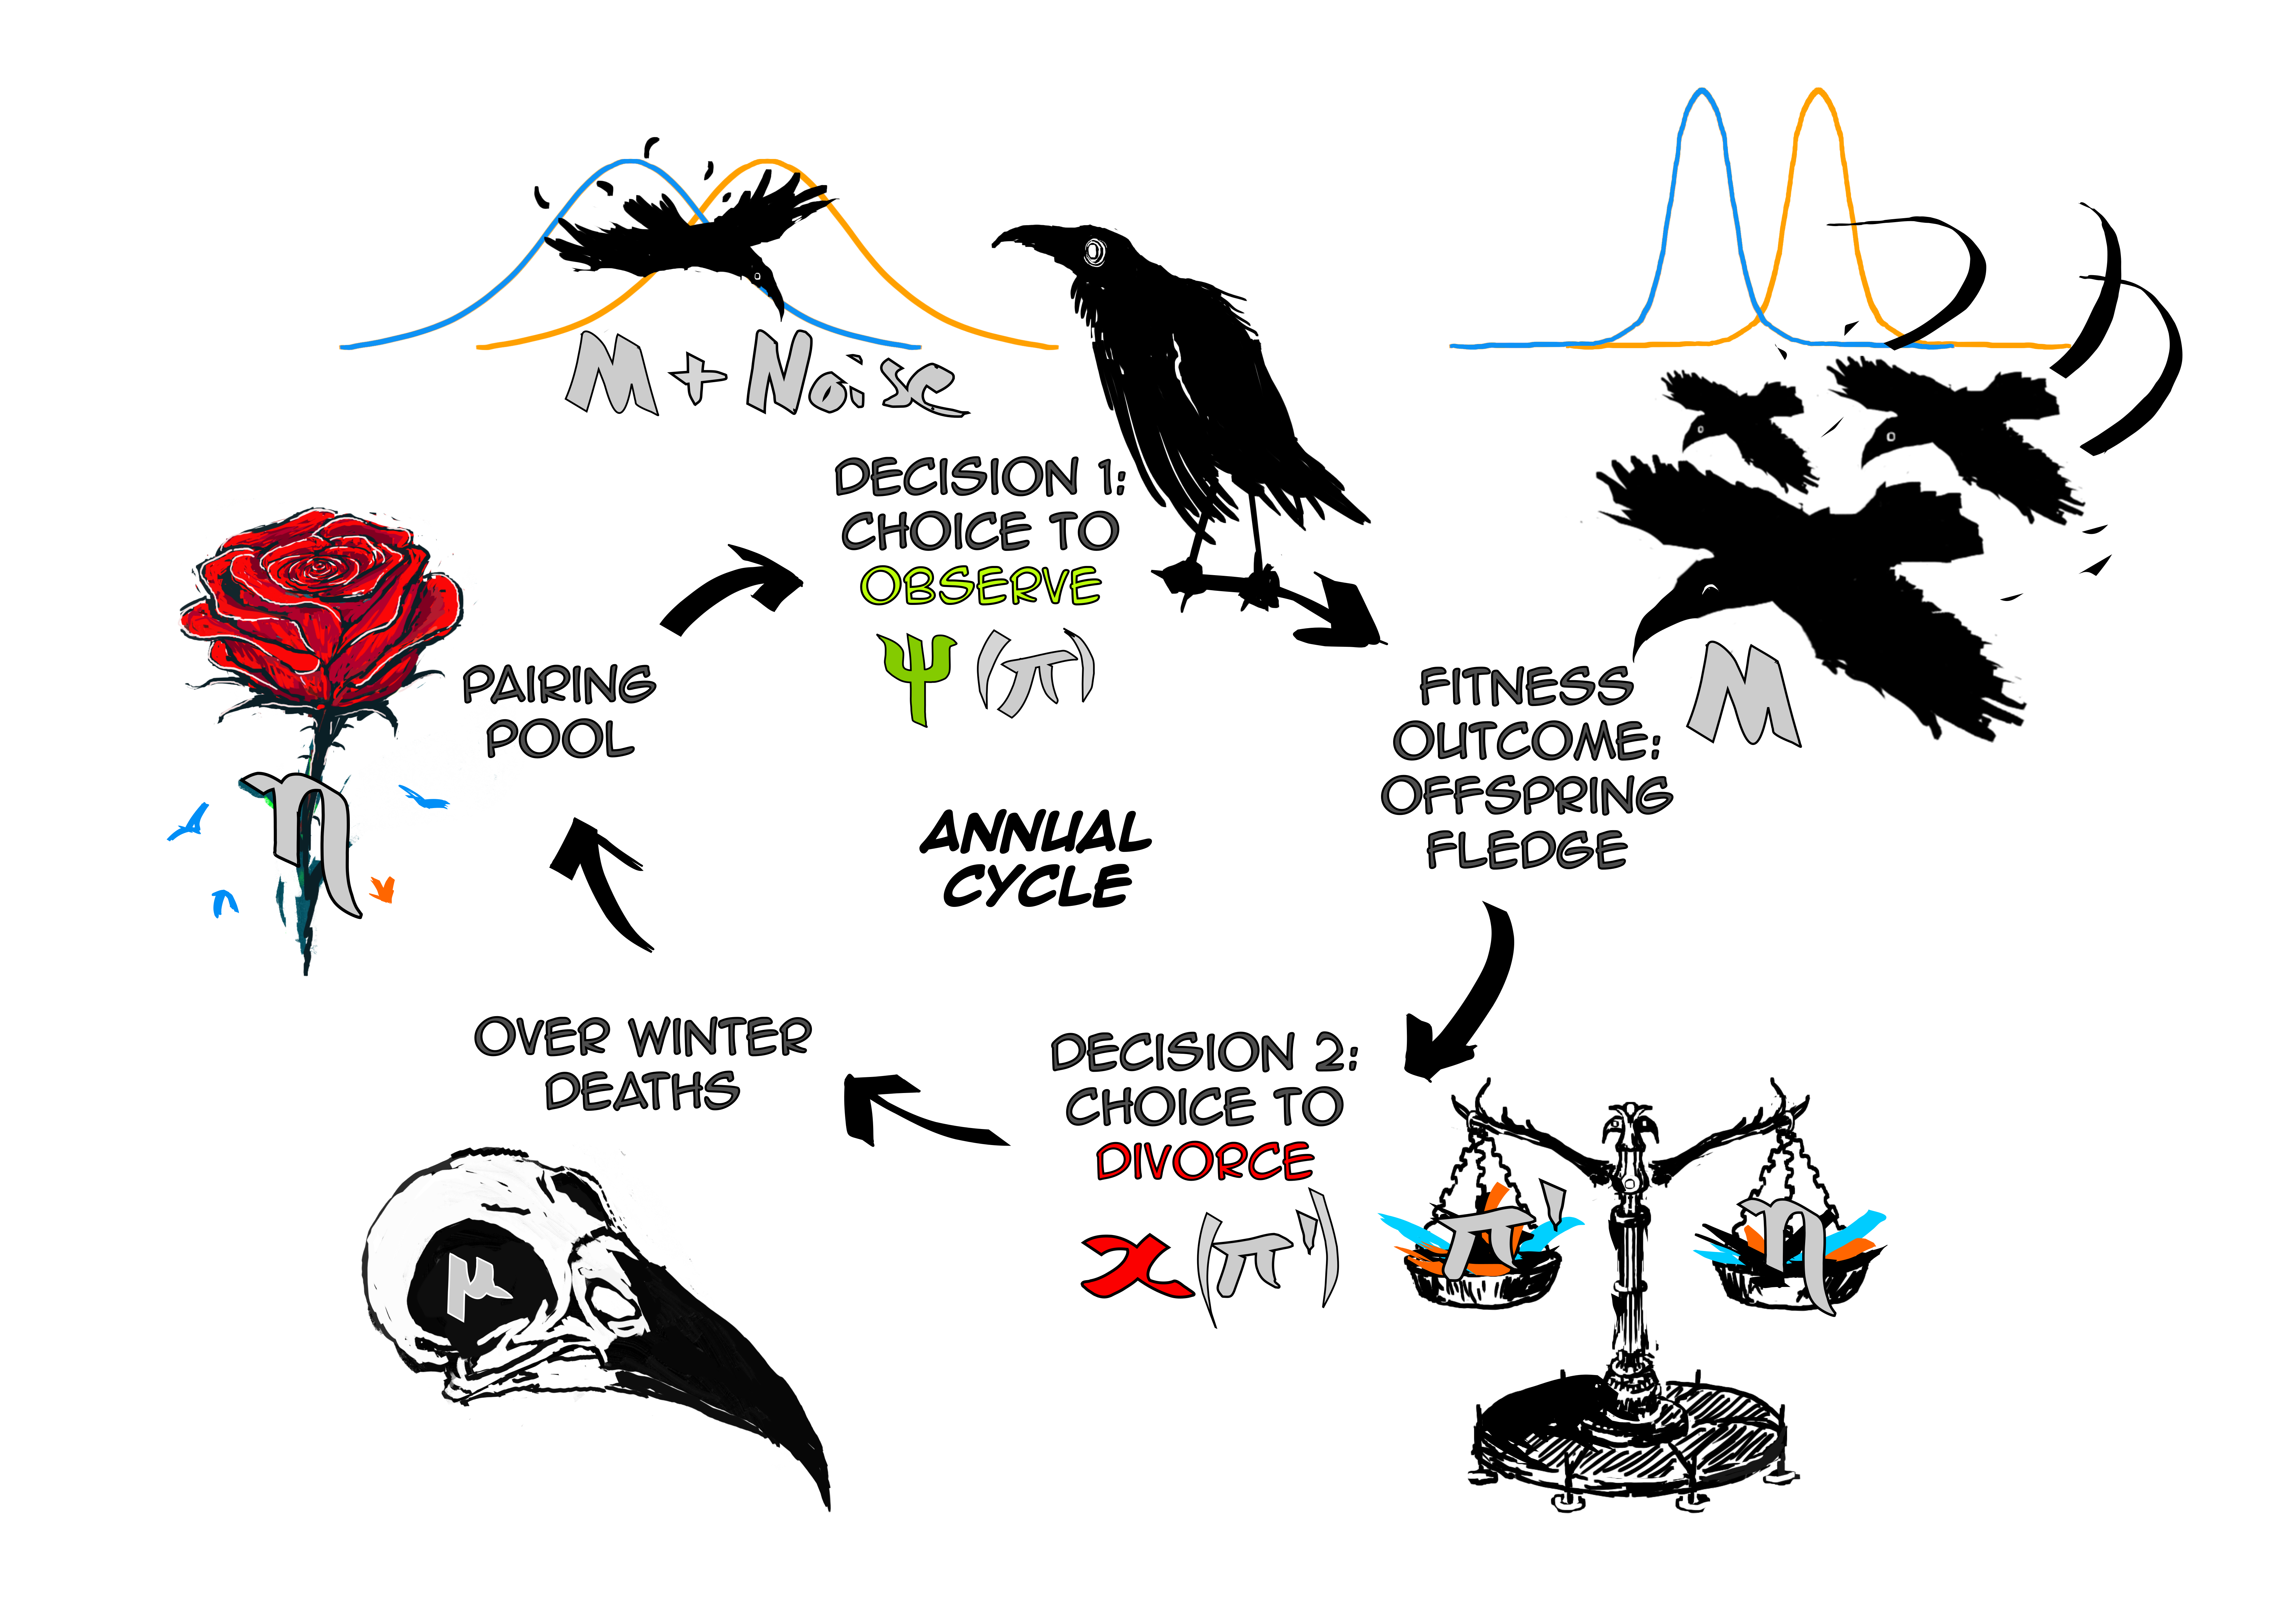
\includegraphics[width=0.8\textwidth]{../figures/drawing2.png}
	\caption{The annual cycle of decision making, with decision 1 being whether to observe their partner, and decision 2 being whether to divorce and enter the pairing pool at the beginning of the next year to form a new pair-bond.}
	\label{Fig:1-2}
\end{figure}

\subsection{Annual Cycle}
A summary of the annual cycle  can be found in Figure \ref{Fig:1-2}. At the beginning of each breeding season all single males and females randomly pair up in the pairing pool, with the distribution of high quality males in the pairing pool being $\eta$. 

The females must then decide whether to observe their partner quality by observing a normally distributed cue of partner quality (for example parental provisioning performance) with which she uses Bayesian updating to generate a posterior belief state $\pi'$. This decision is made using her state-based policy $\psi(\pi)$. This observation may come at an opportunity cost $C_c$  (for example time spent observing takes time away from her own parental provisioning); and/or a mortality cost $C_\mu$ (for example risk of death due to reduced energy reserves). 

Offspring mass at fledging determines the female’s fitness and is an outcome of her and her partner’s quality. So, offspring mass is a less noisy cue of partner quality, which we assume all females gather, with the costs of this being contained within the probability of death between years ($d$). 
\begin{equation}
	M=(1-C_c)a_{f}+a_{m}+\epsilon\label{eq:1}
\end{equation}
Where $ a_f $ is female quality, $ a_m $ is male quality, and $ \epsilon $ is a random variable with a pseudo-normal distribution about 0, with standard deviation $\sigma$.

At the end of the breeding season the female decides whether to divorce and re-enter the pairing pool or commit to the same male. This decision is made using her state-based policy $x(\pi)$. We assume there is no cost of divorce besides the outcome of ending up with a partner of lower quality in the next breeding season. All individuals then have the same probability of dying $\mu$ and are replaced by new unpaired individuals, with a quality distribution $\beta$, making any partner they had also unpaired.

\subsection{Information Use} 
As discussed, to make her decisions, she has a belief state $\pi$ about her partner's quality and we assume the female knows her own quality $a_f$. When she first enters the pairing pool (either after reaching maturity or after divorce), we assume she starts with the pairing pool distribution $\eta$ as her prior belief state $\pi$. She may then each year accumulate greater certainty about her partner's quality by updating this belief state using cues from observations she has chosen to make and from offspring mass at fledging at the end of each year's breeding season. We consider a population in which almost all females use the same resident strategy $(x,\psi)$. As the resident strategy influences the proportion of high quality males that enter the pairing pool, and so prior belief $\eta$, we expect social feedback to occur.

\subsection{Demographic Stability}
As eluded to, the proportion of high quality males in the pairing pool $ \eta $ is influenced by the bottom-up effects of individual decision making, which depend on the states of individuals in the population, which vary over time. We would hope to find that a dynamic system such as this has a stable state to make an easier job of finding the best response strategy for an invading female (see below). To this end, we hope to reach demographic stability by iterating forwards over multiple breeding seasons, assuming that when all individuals are using the same resident strategy the system will approach a stable state, $ \tilde{\eta}_{x,\psi}$. In the Appendix we outline the procedure for doing this. We assume that the population is large and that there are equal numbers of males and females. The initial distribution of the pairing pool and prior of all individuals will be $ \beta $, the proportion of males that are high quality in the population. If there is a singular attractor state of the system, the initial state should not matter. 

\subsection{Evolutionary Stability}
The benefit of having assumed demographic stability is that given some resident strategy $(x,\psi)$, we get a distribution of states and actions in the resident population that will determine the state transition probabilities and prior belief of an invading female. We can then determine the expected fitness outcomes of her actions each year that she lives. At the end of her life she will have zero fitness regardless of her state, so this is the best place to start. We then iterate backwards; in the previous year, if she were of state $\pi_1$ she would have an offspring mass $m_1$ and but if she were of state $\pi_2$ she has greater offspring mass $m_2$. As she will die before she has a chance to produce more offspring her future state is irrelevant so the decision to divorce does not yet matter either. However we go back one year further and perhaps it does, if she has a non zero probability of death between years. As we continue to iterate backwards her decisions may converge on a state based policy that accounts for her expected lifetime fitness outcomes. This stable outcome is the best response to the resident strategy. We assume that this best response strategy will become the new resident strategy. If this does not change the resident strategy then the resident strategy is an evolutionarily stable strategy (ESS) \cite{Smith1982}. When the resident strategy is the ESS, there is no way for a female to alter her policy to improve her expected fitness outcomes. If the resident strategy does change we ought to start again with this new environment, find the demographically stable outcome, and find the next best response. We repeat this process until hopefully the resident strategy does converge on an ESS.

\section{Results}
\subsection{The ESS Divorce Strategy}
The expected fitness outcome in a given year for a female with belief state $\pi$, having used observation strategy $\psi$, is
\begin{equation}
	R(\pi,\psi)=\underset{i}{\sum}m_{i,psi}(\pi P(i|H,I_\psi)+(1-\pi)P(i|L,I_\psi)),\label{eq:16}
\end{equation}
Where $m_{i,psi}$ is the offspring mass at fledging, given message $i$ from $I_M$,observation strategy $\psi$, and it's related opportunity cost on mass $C_O$. Higher values of $\pi$ generates a greater expected offspring mass. Using the calculations outlined in the appendix we found that for a given resident strategy and life history, the decision-relevant state of the pairing pool $\eta$ approaches a unique value. We use this to determine the fitness outcome of entering the pairing pool and as there is no cost to divorce per se, only a cost in bad decision making with respect to the belief state $\pi$, we find that the ESS divorce strategy is rather straightforward. Given that belief state $\pi$ determines the probability that the male is high quality, $\eta$ is the probability that their partner post-divorce will be high quality, and expected fitness outcomes increase with Male quality in a given year, the female should divorce if 
\[
\pi<\tilde{\eta},
\]
To put it simply, the female chooses when it maximises the expected value of $\pi$, as this maximises $R(\pi,\psi)$. Hence we see that the divorce threshold and the stable pairing pool state $\tilde{\eta}$, are one and the same. Thus any factor that effects the stable state of the pairing pool also has an effect on the behaviour of females.
 

\subsection{The ESS Observation Strategy}

The optimal observation strategy is not so straightforward to solve for. The use of an observation does not change the expected value of the female's posterior belief state, instead it changes the belief state for the better for proportion $\pi$ of the females and for the worse for the rest, but for the latter they can use divorce to remedy this. Expected amount of change depends on the amount of uncertainty in her prior belief and the informativeness of the observation. To find the Observation ESS we first find the best response to a resident strategy with pairing pool distribution $\eta$, assuming optimal divorce decision making 
\begin{equation}
	\hat{b}(\psi)(\pi)=\underset{\psi}{argmax}\{R(\pi,\psi)+\underset{k}{\sum}(1-C_{\mu}\psi)\mathbb{P}(\pi'=k|\pi,\psi)\underset{}{max}\{(H_{D}(\eta),H_{C}(\pi'))\}\}, \label{eq:26-1}	
\end{equation}
where $\mathbb{P}(\pi'|\pi,\psi)$ is the state transition probability from the prior belief state $\pi$ to the posterior belief state $\pi'$ given observation strategy $\psi$, $H_{D}(\eta)$ is the fitness outcome of divorce given $\eta$ calculated for a given resident strategy (outlined in Appendix), and $H_{C}(\pi')$ is the fitness outcome of committing to the male given posterior belief state $\pi'$. $R(\pi,\psi)$ includes the effect of the opportunity cost of the observation, $\mathbb{P}(\pi'|\pi,\psi)$ gives the effect of informativeness, and $C_\mu \underset{}{max}\{(H_{D}(\eta),H_{C}(\pi'))\}$ gives the usability of the information received given the risk of death when making the observation and the actions available.
To find the evolutionary stable strategy we iterate over invasions of best response strategies until
\begin{equation}
	\hat{b}(x,\psi)=(x,\psi).\label{eq:26}
\end{equation}
What we find in the baseline case (see Figure \ref{fig:2}) is that the observations are most beneficial when the female has high uncertainty in her prior belief state, and when her belief state is near to the divorce threshold set by $\eta$, because this is when the probability of a decision-relevant change in belief state is most likely. We also find that as females grow older observation and divorce rates go down, as their certainty that they are paired with a high quality male goes up, plateauing due to the turnover rate of the population limiting the proportion of females that can reach certainty.

\begin{figure}
\centering
\includegraphics[width=0.8\textwidth]{../figures/baseline.png}
\caption{Divorce and information use with age, with baseline parameters: Abundance of H ($ \beta=0.5 $), Mortality rate ($ \mu=0.2 $), Mass information structure ($ \delta=10, \sigma=5 $), Observation Noise ($ Noise=1 $), Opportunity Cost ($ C_o=0.005 $), Mortality Cost ($ C_m=0 $). The panels on the left show the relationship between female age and the probability that she will observe (top) and divorce (bottom) low and high quality males. The panels on the right show the ESS observation policy $\psi*$ (top), ESS divorce policy $x*$ (bottom) for all females, with the grey areas indicating where the action to observe (top) and divorce (bottom) will be chosen.}
\label{fig:2}
\end{figure}

\begin{figure}
	\centering
	\begin{subfigure}{.5\textwidth}
		\centering
		\caption{Low difference and variance ($\delta = 10$, $\sigma = 5 $)}
		\includegraphics[width=1.\linewidth]{../figures/baseline.png}
		\label{fig:sub3}%
	\end{subfigure}%
	\begin{subfigure}{.5\textwidth}
		\centering
		\caption{High difference and variance ($\delta = 14$, $\sigma = 7 $)}
		\includegraphics[width=1.\linewidth]{../figures/detectability.png}
		\label{fig:sub4}
	\end{subfigure}%
	\caption{Varying both $\delta$ and $\sigma$, with all else the same as the baseline parameters, we find that information use and divorce rates (and their respective strategies) are the same when detectability is the same.}
	\label{fig:4}%
\end{figure}

\begin{figure}
	\centering
	\begin{subfigure}{.5\textwidth}
		\centering
		\caption{No Observations}
		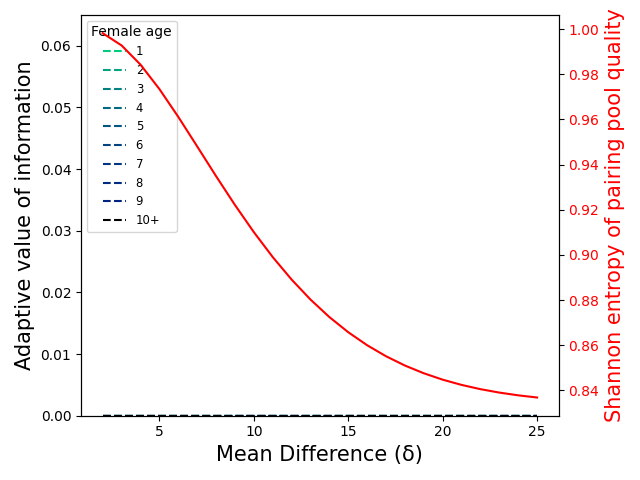
\includegraphics[width=1.\linewidth]{../results/Mean0/canons.png}
		\label{fig:sub1}
	\end{subfigure}%
	\begin{subfigure}{.5\textwidth}
		\centering
		\caption{Observations}
		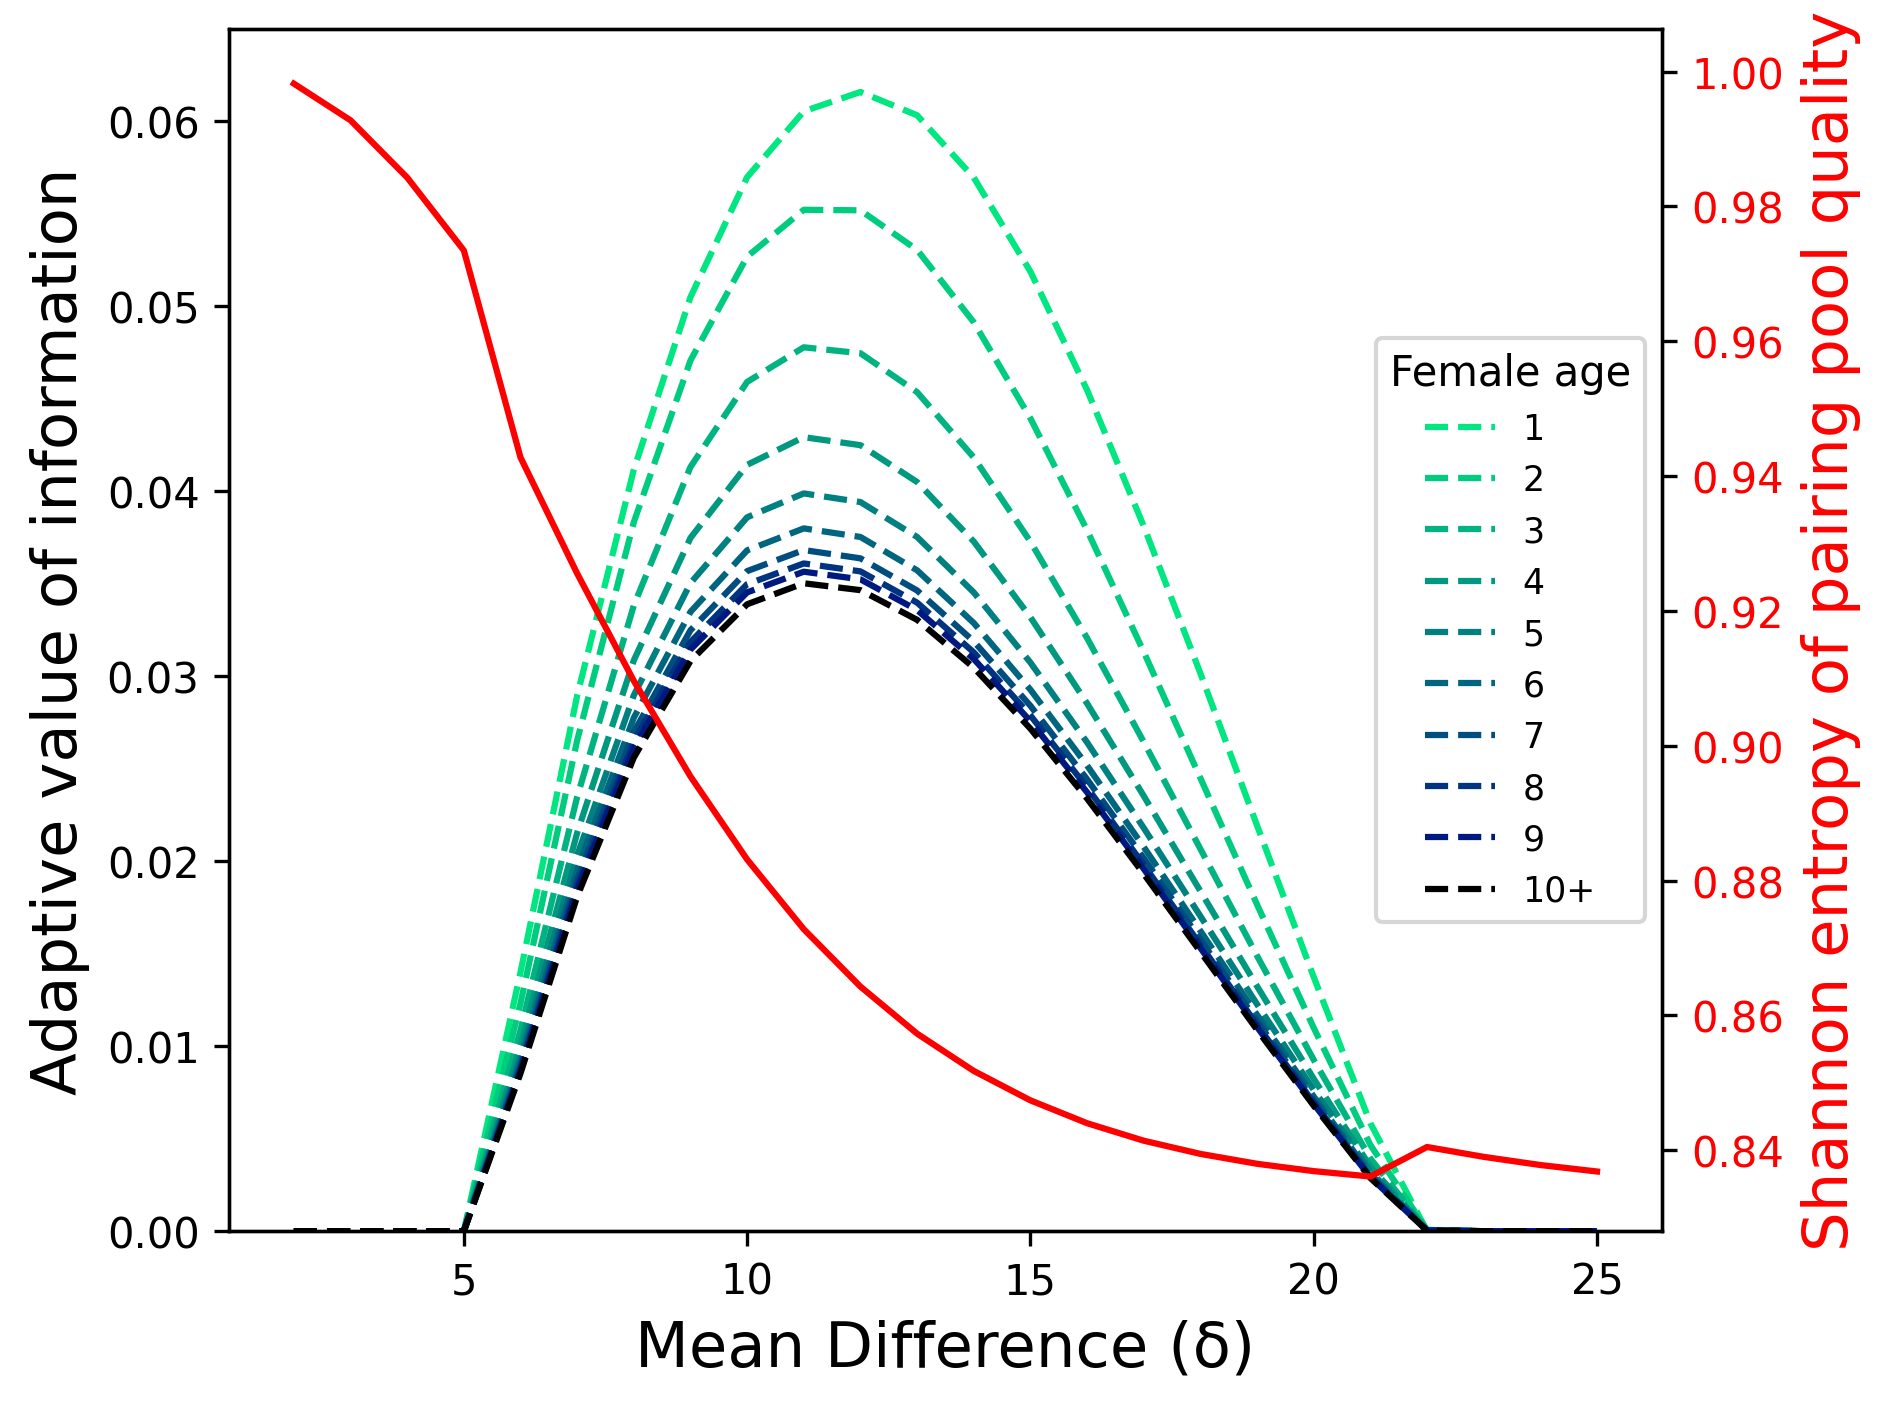
\includegraphics[width=1.\linewidth]{../results/Mean2/canons.png}
		\label{fig:sub2}%
	\end{subfigure}%
	\caption{Varying mean difference $\delta$ between low and high male quality, with all other parameters at the baseline values. We use Shannon Entropy as a measure of the uncertainty in the pairing pool, highest when $\eta = 0.5$. Feedback of information use on uncertainty in the pairing pool is demonstrated by comparison between the entropy curves for these two graphs. As uncertainty decreases with an increase in $\delta$, the informativeness and so value of observations decreases. At very low values of $\delta$, observation cues are very low in detectability (see section 3.3.1) and so uninformative and less valuable despite the high uncertainty.}\label{figLabel}
	\label{fig:3}%
\end{figure}


\begin{figure}
	\centering
	\begin{subfigure}{.5\textwidth}
		\centering
		\caption{$C_O = 5e-3, C_\mu = 0$}
		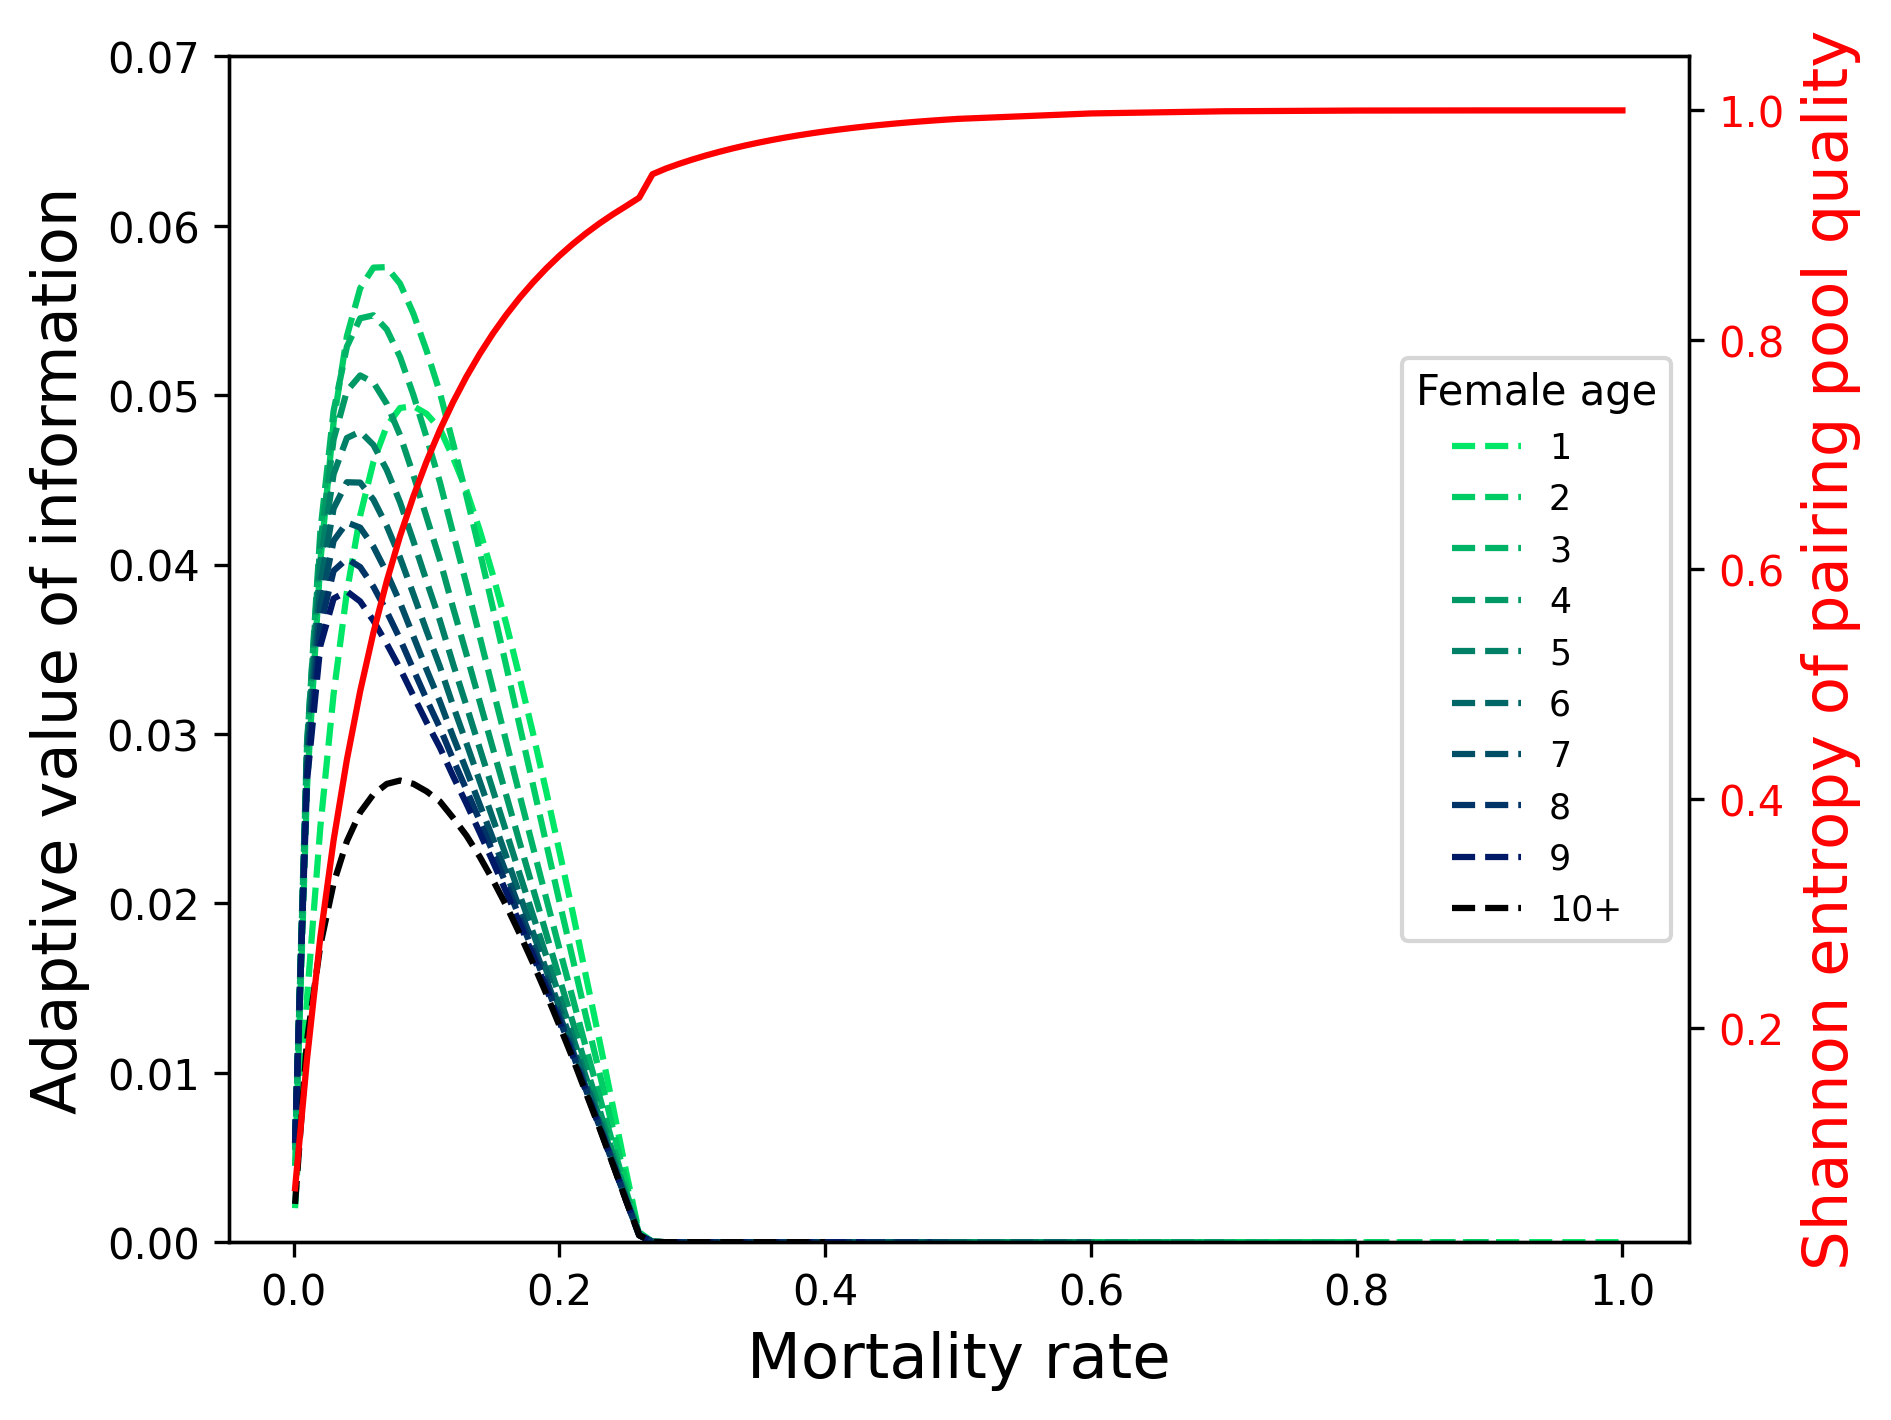
\includegraphics[width=1.\linewidth]{../figures/mortCo.png}
		\label{fig:sub5}
	\end{subfigure}%
	\begin{subfigure}{.5\textwidth}
		\centering
		\caption{$C_O = 0, C_\mu = 5e-4$}
		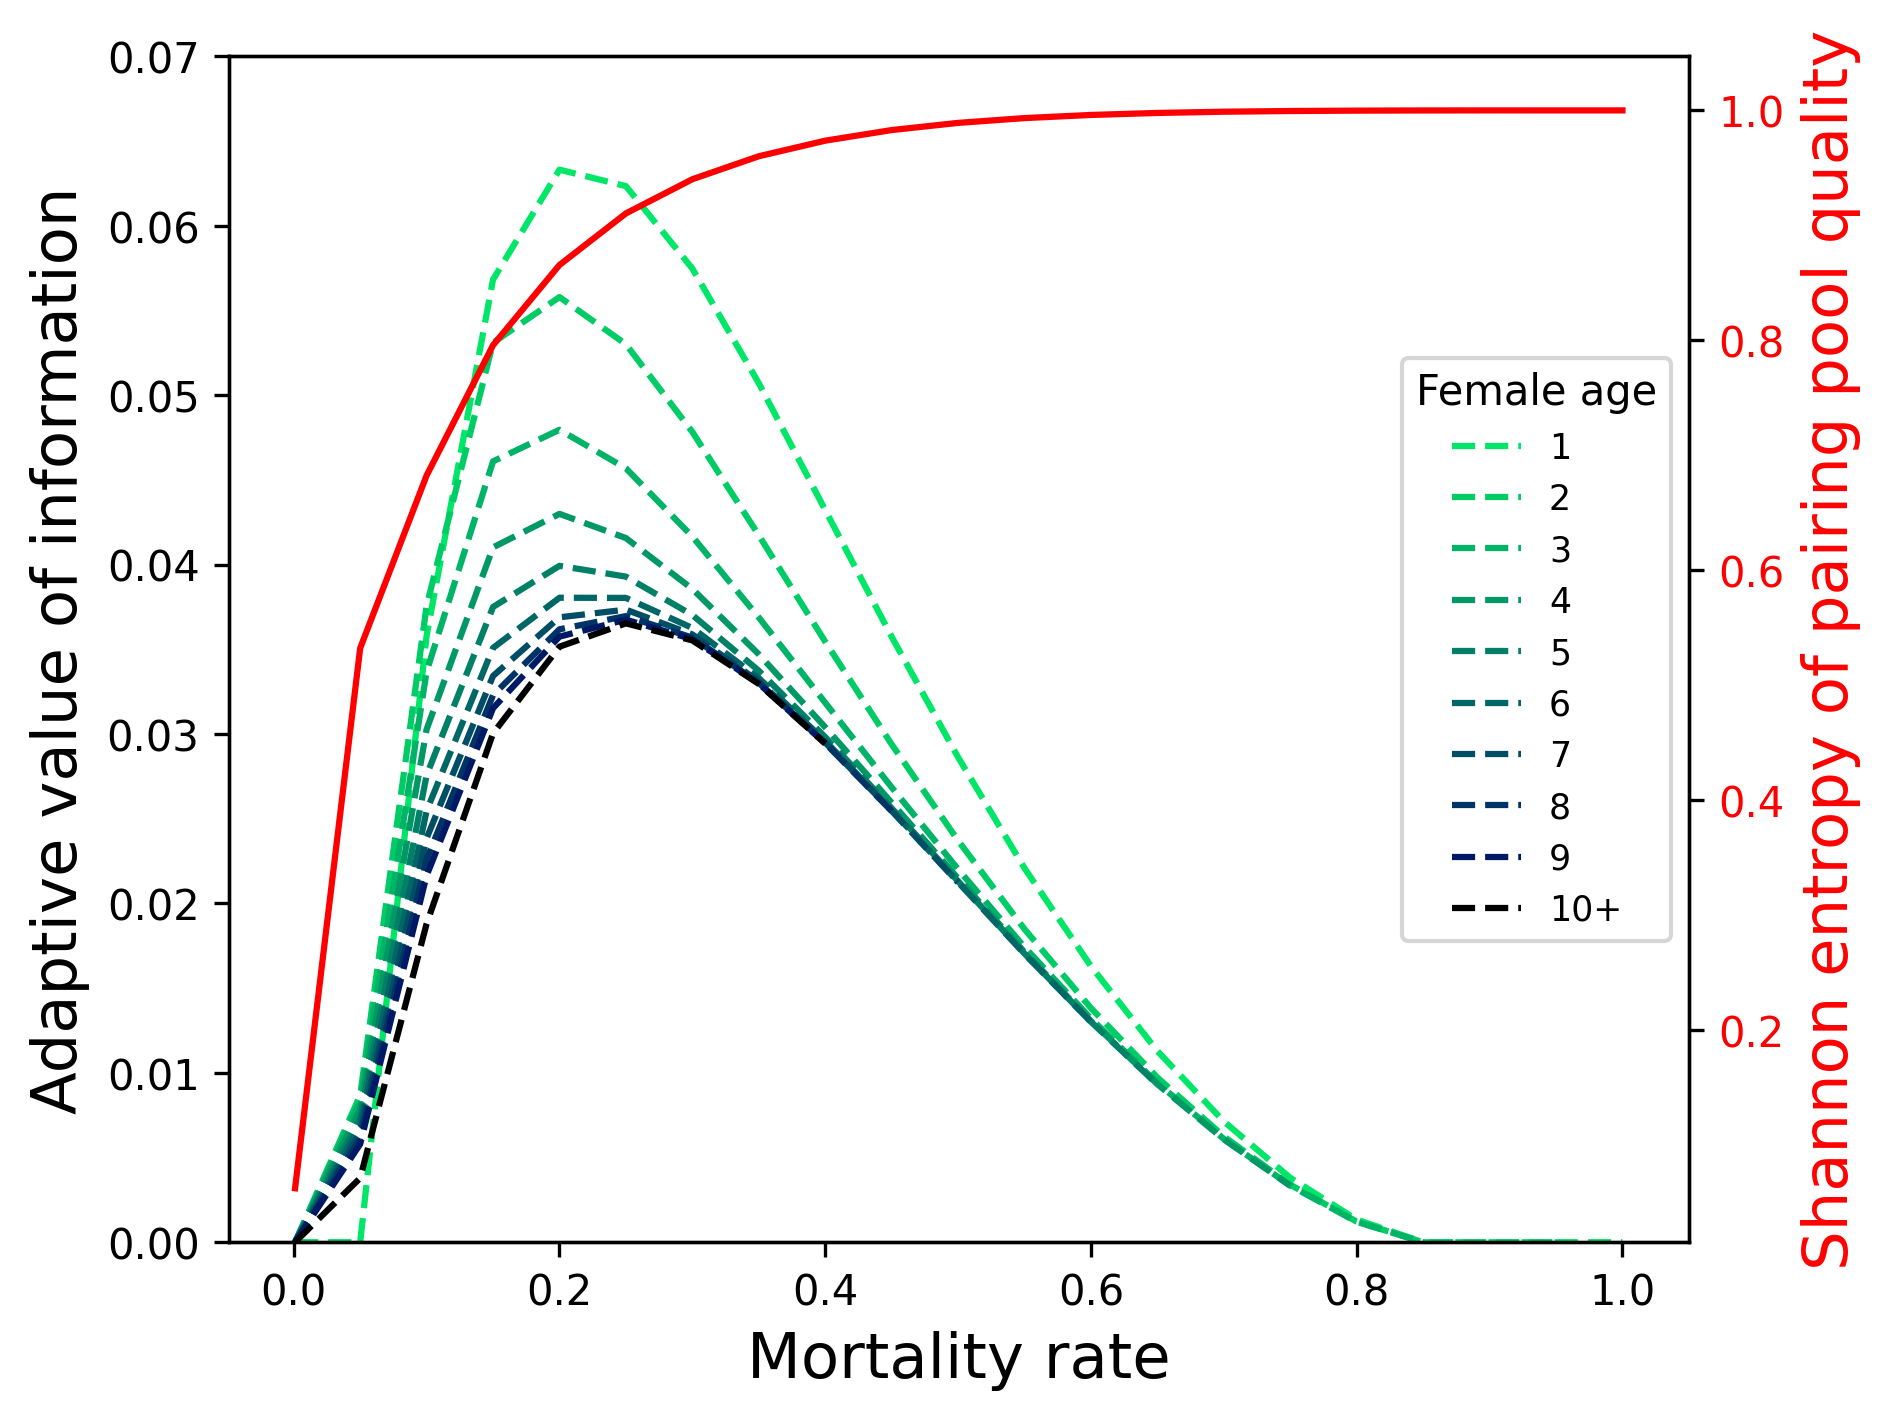
\includegraphics[width=1.\linewidth]{../figures/Mortmu2.png}
		\label{fig:sub6}%
	\end{subfigure}%
\caption{Information use and the nature of the costs for different mortality rates. With opportunity costs the value of information is tightly distributed at very low mortality rates, but value approaches zero as mortality rate approaches zero, as uncertainty approaches zero. With mortality costs we see value of using information for a wide range of mortality rates and the elimination of information value for very low mortality rates. }
\label{fig:5}
\end{figure}

\begin{figure}
\centering
\begin{subfigure}{.5\textwidth}
	\centering
	\caption{$C_O = 5e-3, C_\mu = 0$}
	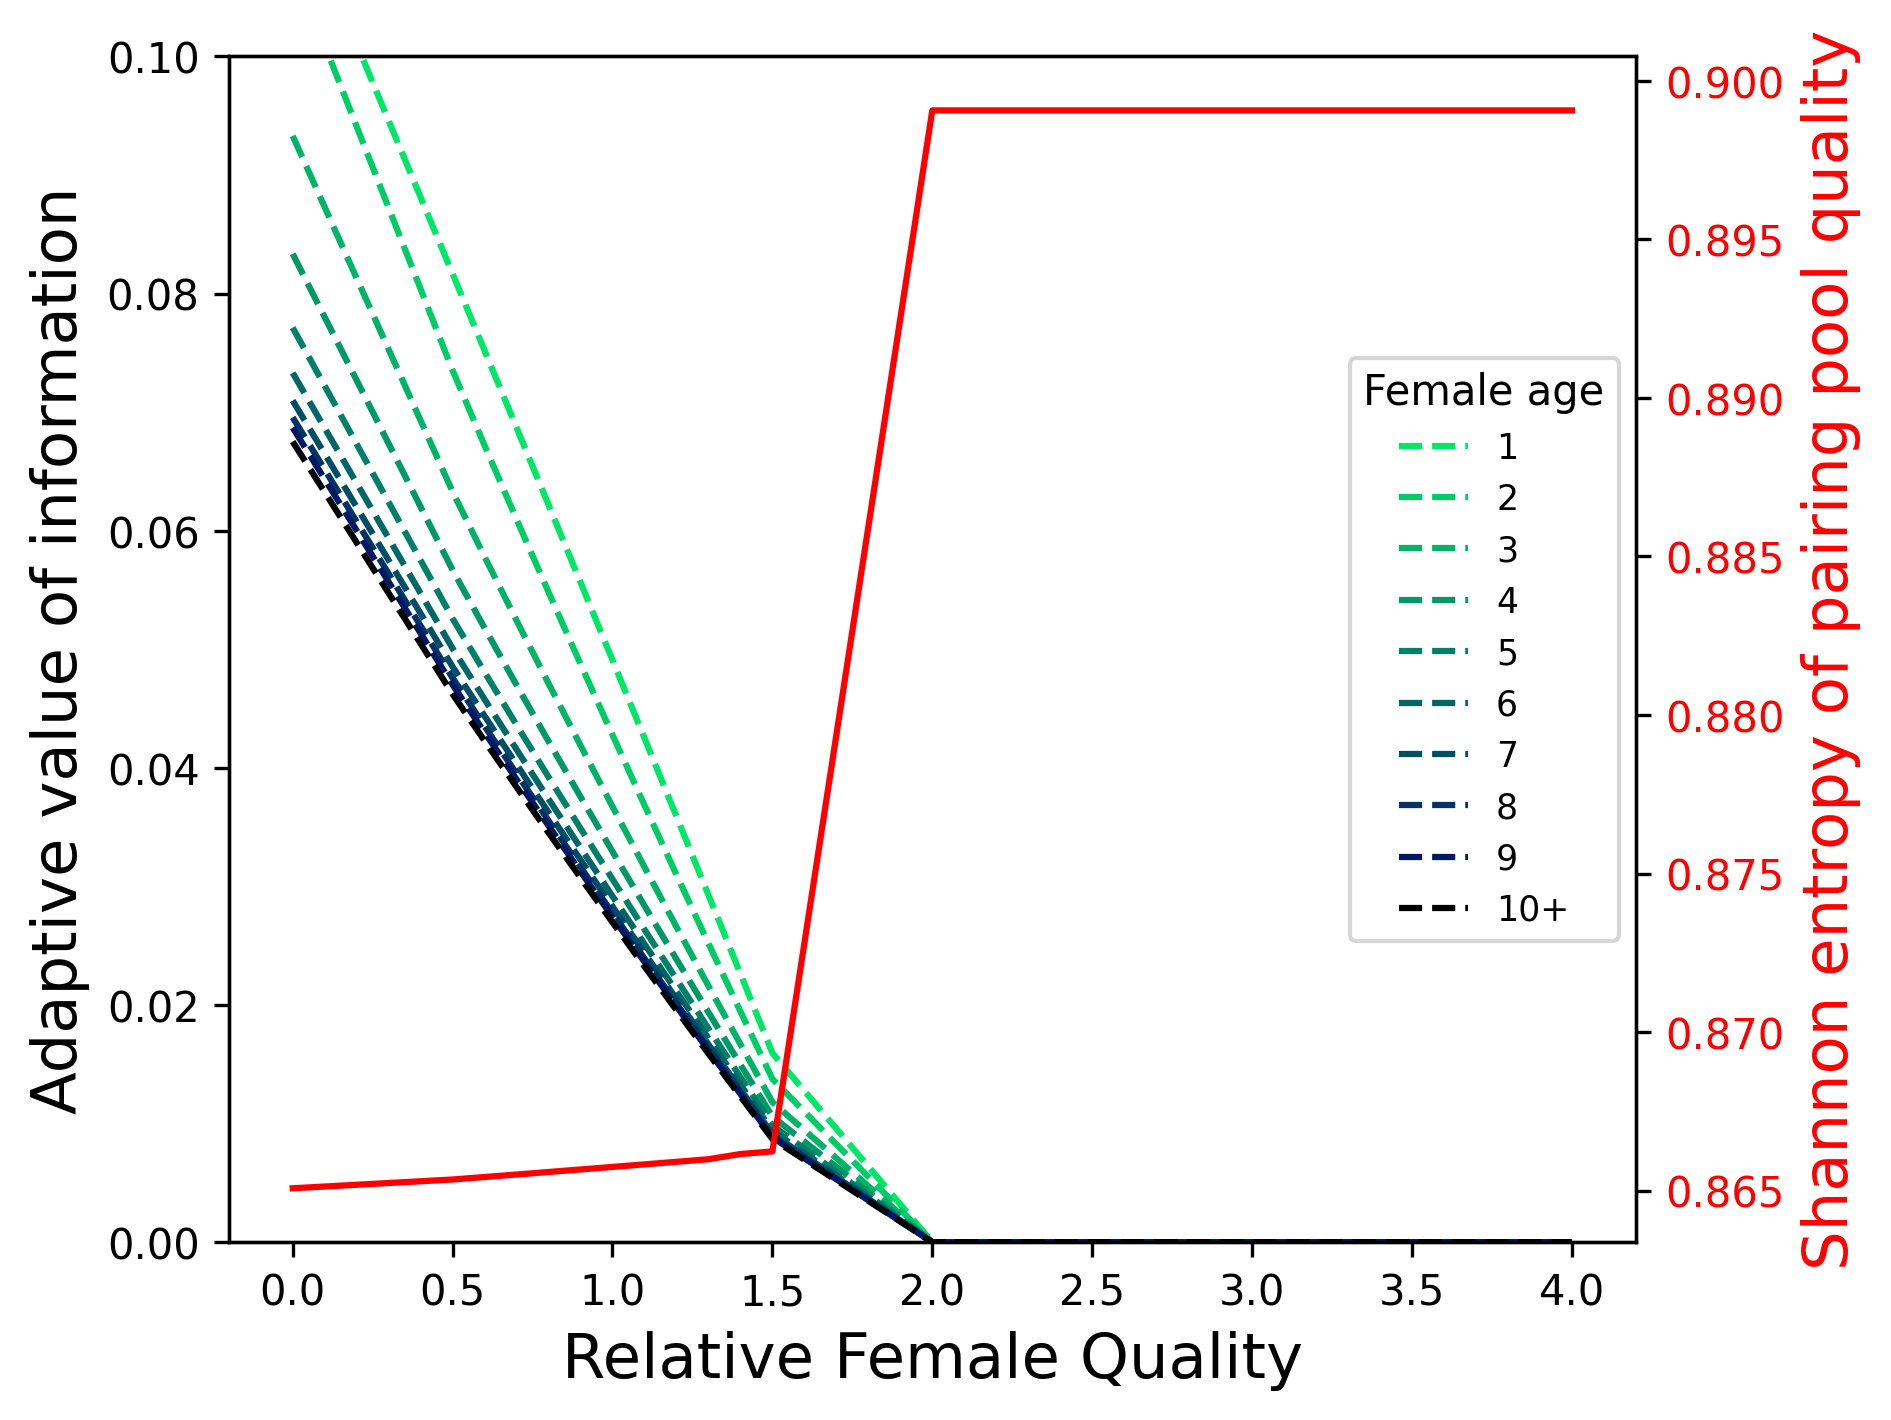
\includegraphics[width=1.\linewidth]{../figures/FemQual.png}
	\label{fig:sub7}
\end{subfigure}%
\begin{subfigure}{.5\textwidth}
	\centering
	\caption{$C_O = 0, C_\mu = 5e-4$}
	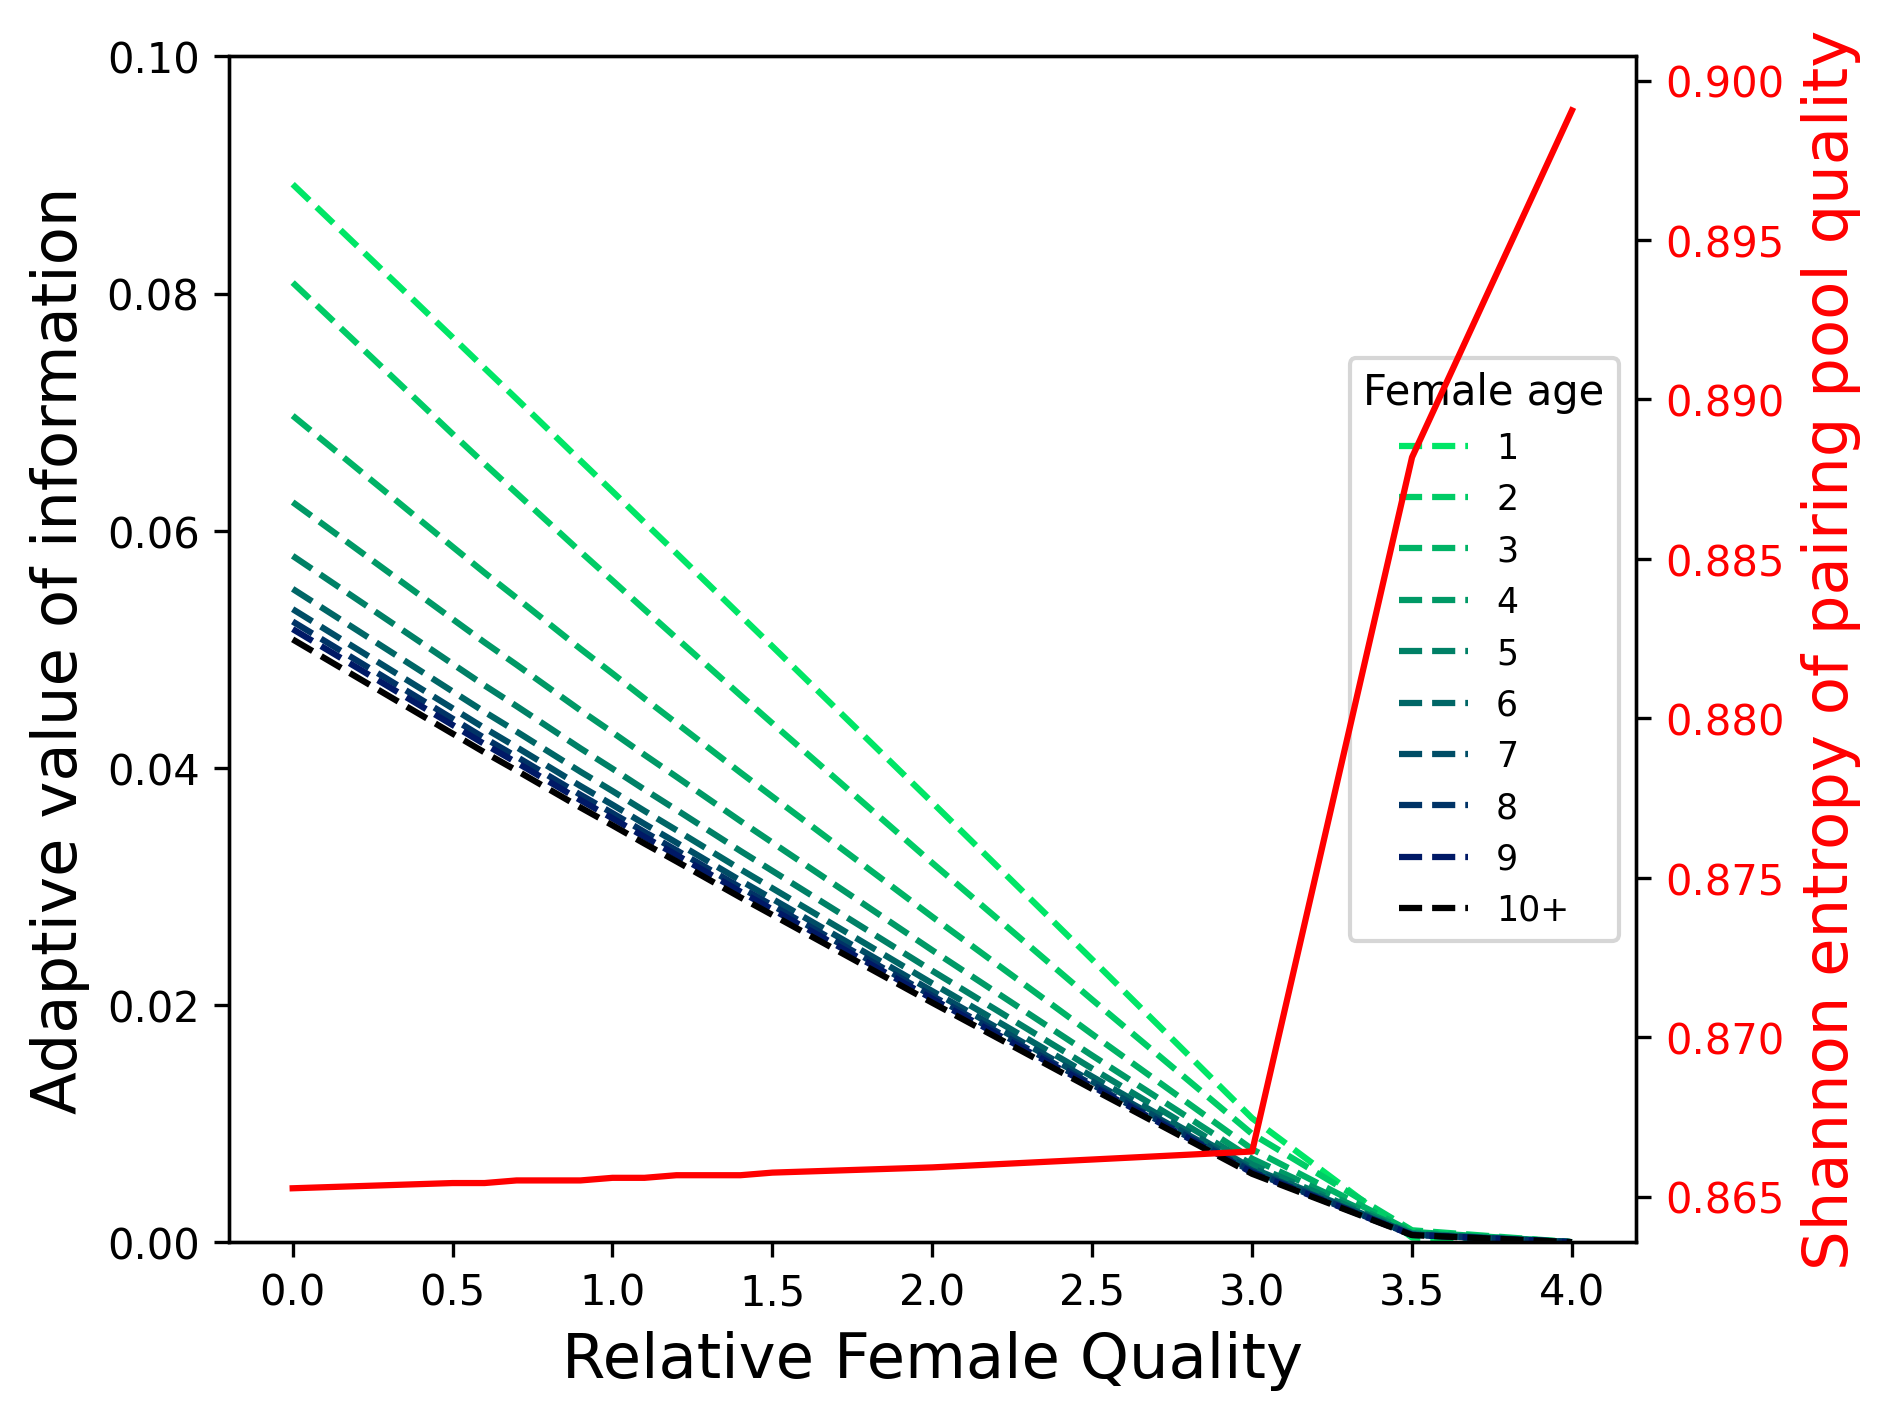
\includegraphics[width=1.\linewidth]{../figures/FemQualmu.png}
	\label{fig:sub8}%
\end{subfigure}%

\begin{subfigure}{.5\textwidth}
\centering
\caption{$C_O = 0, C_\mu = 5e-4$, high female quality}
\includegraphics[width=1.\linewidth]{../figures/Mort_Co_fvH.png}
\label{fig:sub9}%
\end{subfigure}%
\begin{subfigure}{.5\textwidth}
\centering
\caption{$C_O = 5e-3, C_\mu = 0$, high female quality}
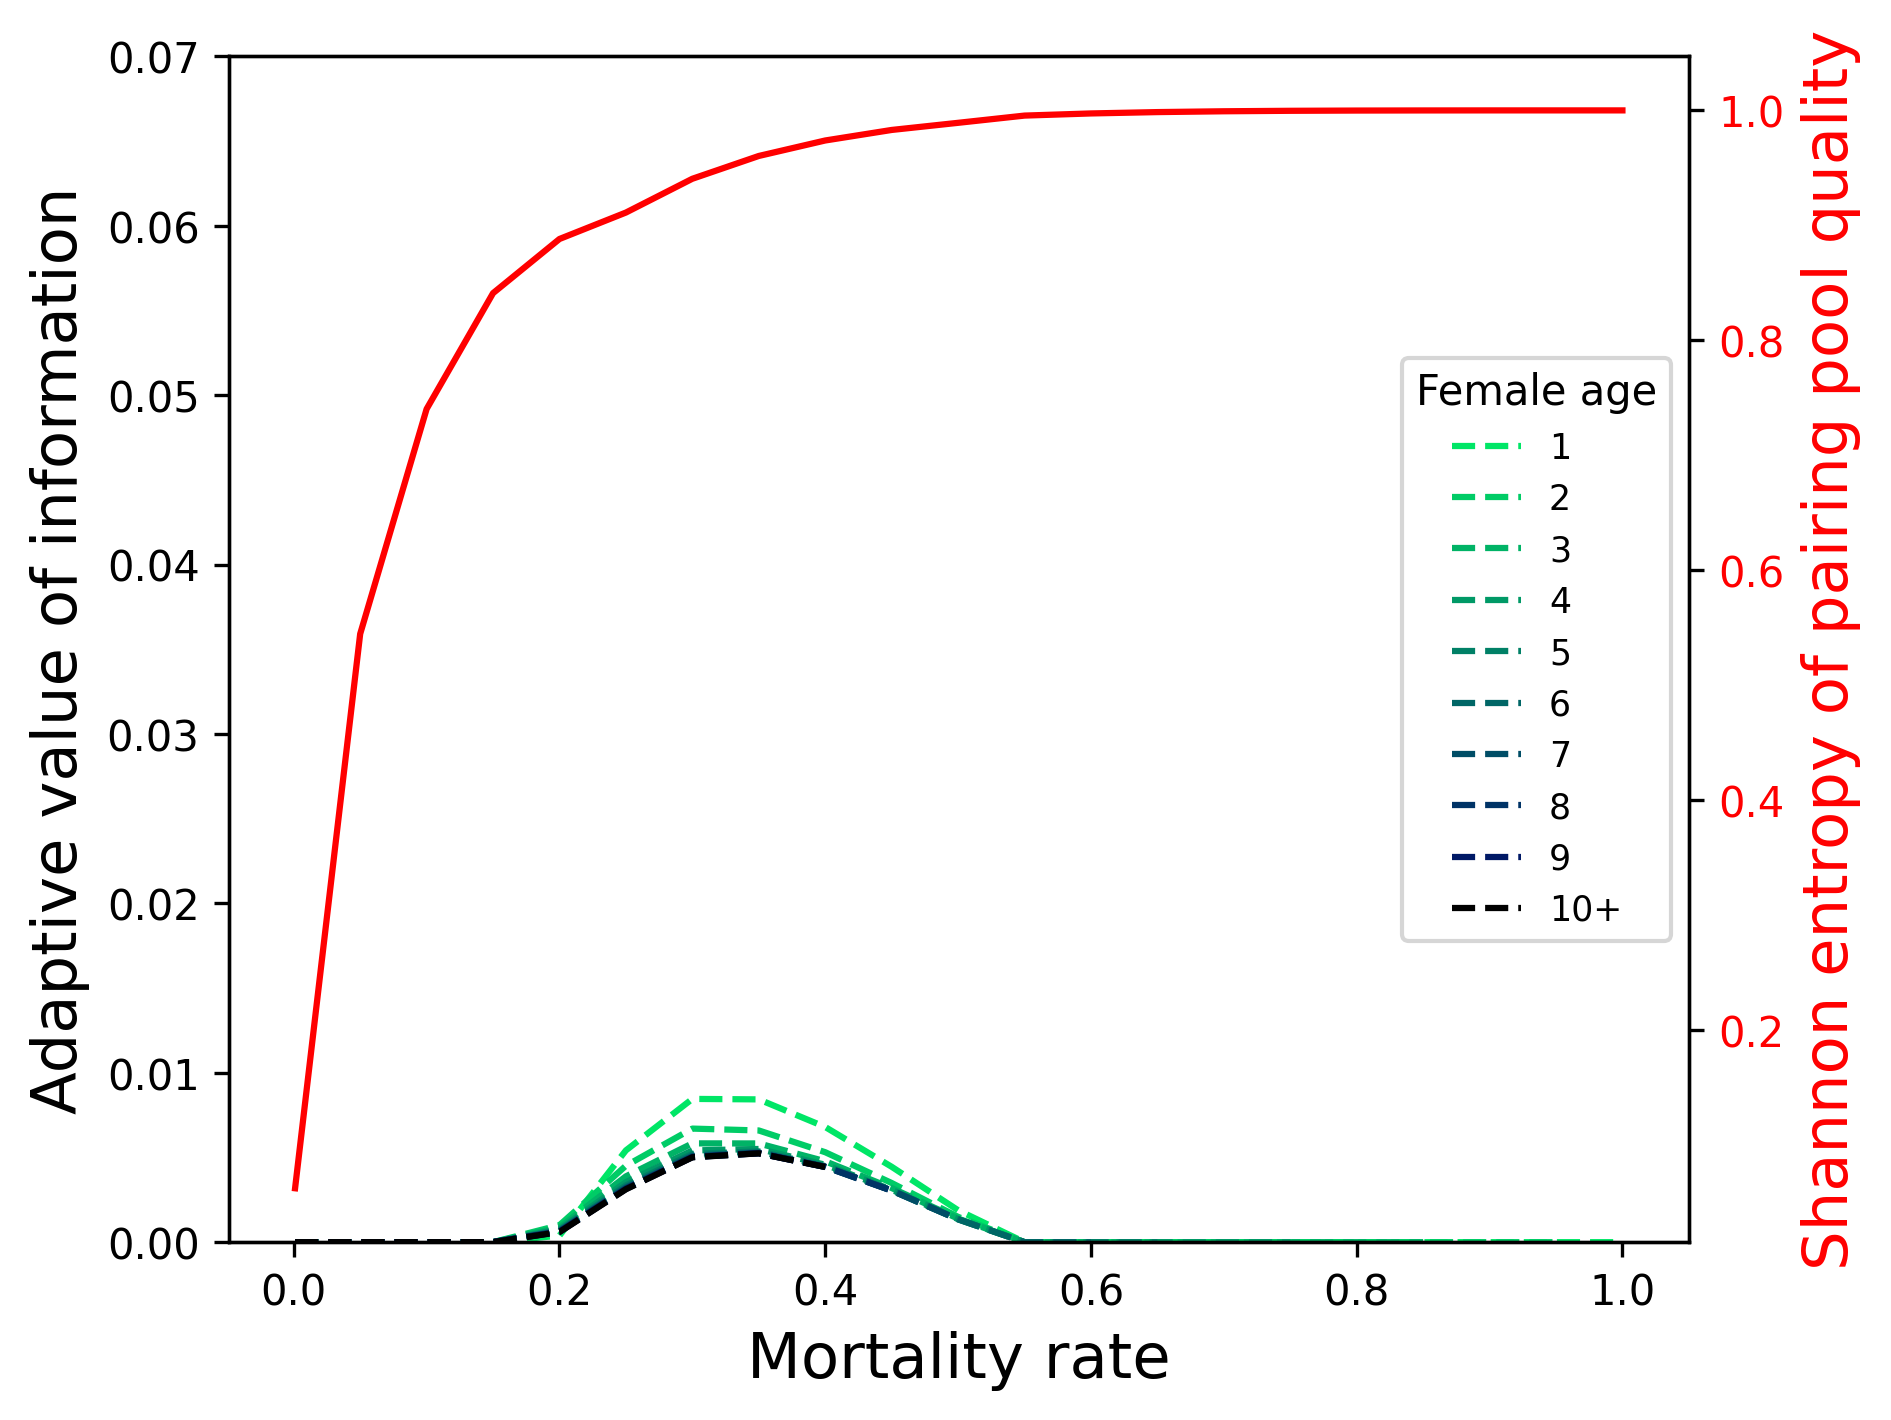
\includegraphics[width=1.\linewidth]{../figures/FemMort.png}
\label{fig:sub10}%
\end{subfigure}%
\caption{Female Quality determines and the value of information and interacts with the cost-lifespan dynamic. \ref{fig:sub7} Low quality cooperators ought to gather information to improve outcomes; \ref{fig:sub8} high value cooperators ought to prioritise their own contributions and their lifespan; \ref{fig:sub9},\ref{fig:sub10} higher female quality exaggerates the nature of the costs.}
\label{fig:6}
\end{figure}

\subsection{Parameter Explorations}
\subsubsection{Information Structures}

Ultimately we find that the mean difference and the variance have interchangeable effects via the detectability of the cue \citet{leavell2019cognitive,Egan1975}
\begin{equation}
	d'=\dfrac{\delta}{\sigma}
\end{equation} 
Where, in the case of the mass cue, $\delta$ is the mean difference in offspring mass between high and low quality males and $\sigma$ is still the standard deviation of the normal distribution. As the cue in this case is itself the offspring mass, the fitness benefit is the same for a given detectability value irrespective of what combination of mean difference and variance gave that same detectability and so we can expect the same behavioural outcomes (see Figure \ref{fig:4}). We can see the effect of detectability on information value in Figure \ref{fig:sub2} discussed below.

\subsubsection{The social information feedback loop}
We see in \ref{fig:sub1} that lower cue noise means reduced uncertainty about the pairing pool. When we allow for the use of observations \ref{fig:sub2}, we see that the low uncertainty in the pairing pool at low cue noise means a reduced value of observation, reducing the informativeness of the cue just as high cue noise does. We also see that where observations are made this auxiliary use of cues further reduces social uncertainty (see the difference in the entropy curve between \ref{fig:sub1} and \ref{fig:sub2}) which generates further negative feedback on the value of observations.

\subsubsection{Lifespan}
We find that the relationship between mortality rate and information use is complex. With a greater lifespan (low $ \mu $) there are more seasons in which to reap the benefits of a high quality mate but also fewer seasons in which there is sufficient uncertainty to be resolved, and crucially, less uncertainty in the pairing pool to resolve. So we see that information value is maximal at intermediate mortality rates (see Figure \ref{fig:5}), however the nature of the costs matter. If there is an opportunity cost $C_O$, the influence of the cost is greater for short lived species for whom that cost impacts a greater proportion of any given breeding season. If there is a mortality risk $C_\mu$, the influence of the cost is greater for long lived species as they have a more years of reproduction to lose out on by dying.

\subsubsection{Female Quality}
The opportunity costs of observation are proportional to female quality and thus to the value of information (see figure \ref{fig:sub7}). With mortality costs only, although the link between quality and the costs are less obvious, we still see a similar but weaker effect of female quality on information value (see figure \ref{fig:sub8}). This is because high quality females benefit more from a long life of uncertainty as this uncertainty has a smaller relative effect on their fitness outcomes, and so we also find that the greater the mortality risk the more information value depends on female quality. For this reason, if we increase female quality, we also see an exaggeration of the effect of mortality costs on long lived species use of social information in this context (see Figure 7).

\section{Discussion} 
\subsection{Social Information Loops}
As with the divorce model by \citet{Lerch2022}, uncertainty and social feedback moderate individual decision making, and our model shows that this social feedback also has influence on uncertainty and information use. More information use means less uncertainty. Less uncertainty means information is less valuable, all else being equal. If information is affordable and likely to change decision making for the better, everyone ought to use it, but if they do they will reduce its value if competing for a limited resource (even if the resource has some rate of replenishing). The less uncertainty is in the system, the more detectable the cue has to be to be informative and so the more detectable or affordable it has to be to be worth using. This insight may explain the findings of \citet{Botero2012}, that rates of infidelity are higher amongst monogamous birds living in low predictability environments, increasing uncertainty of male quality, and so increasing the likelihood of any information to bring their partner quality belief above their threshold for promiscuity if they have one.

\subsection{Lifespan}
It was shown by \citet{McNamara1996a} that lifespan and costs have complex effects on optimal divorce strategies, and we find similar and some novel effects for optimal information use in this context. The new insight is that the longer lived the species the less uncertainty is in the system and so the informativeness of observations goes down reducing optimal levels of information use, but a longer life also means more breeding seasons in which to reap the benefits of certainty, and so information value is greatest at intermediate lifespans. We also show much like in \citet{McNamara1996a} that opportunity costs and mortality costs differ qualitatively in effect as a result of their impact on lifetime usability. Mortality costs reduce information value by eliminating the opportunity to use it indefinitely, meaning the cost is greater for longer lived species and higher quality individuals (see below). Opportunity costs reduces fitness outcomes in a given season, and so as lifespan increases this fitness cost becomes smaller relative to the life time fitness of the organism, while the information gained is used until death or divorce. However, the benefit of the information gained also goes down with age as there have been many years in which to passively gather offspring mass information. In the case of mortality costs, this means that long lived species no longer benefit from observations. So while we predict that long lived species will use more information in general, they will differ in the kinds of information they exploit, generally being more risk averse when it comes to mortality costs. 

\subsection{Cooperation and Uncertainty}
 The results with respect to female quality have a more general interpretation, the less uncertain you are of your own influence on your fitness outcomes the greater the value of social information. The significance of this insight for mate choosiness in contexts where lower contribution affords more numerous matings is not obvious but it may well be a counter balancing force. If females are uncertain about their own quality it becomes more risky to rely on their own contributions. Females ought to invest more in information, for the purpose of finding the best mates, when they believe they contribute less to offspring quality at independence. If how much you contribute is itself a choice of effort, high costs of information or low uncertainty may select for high effort, but high effort may in turn increase uncertainty in the pairing pool. It would be interesting to extend the model so that quality is determined by an effort strategy, perhaps greater effort would be a method of managing uncertainty. This also suggests that if males have low contribution to offspring mass relative to females, it benefits them to gather information and be choosy, so much like the model by \citet{Barta2002} females may reduce their effort so as to encourage the male's effort, as our model shows this reduces the value of observation and so the males capacity to make strategic selfish decisions. If events occur so as to force reduced effort, the value of information goes up. Or if females can use phenotypic plasticity (conditional on other sources of information) to increase their quality (and certainty of quality) over time, uncertainty from extrinsic sources such as male quality becomes insignificant to them.

\subsection{Signalling in Two-sided Divorce}
 Giving the males the option to divorce and observe too would likely both increase the proportion of high quality males in the pairing pool (increasing the value of information) but would also generate a new source of social uncertainty. Males gathering information at an opportunity cost will contribute less to offspring mass, and vice versa for females. This may reduce the informativeness of offspring mass as a result of strategic uncertainty \cite{Bikhchandani2013}, uncertainty about the actions of others, in this case about what opportunity costs were paid and whether they will continue to be paid in the future. One plausible outcome is that high quality females have less to gain from observations and so will express reliable cues of their quality, while low quality females may actually exaggerate their low quality as a trade-off to find high quality males. Another less efficient outcome is that the strategic uncertainty will be self perpetuating (at least for the young) because there is more uncertainty to be reduced, and everyone trying to reduce it just generates more uncertainty. Finally it may even be that it benefits one sex to signal honestly (because the uncertainty does not matter to them) and the other to be choosy, particularly if there are sex differences in mean quality (differences in parental contribution), in which case, the sex whose quality matters less should be more choosy, which could select for male choosiness in many systems.
 
\subsection{Conclusion}
In a simple social interaction such as this, competition to choose high quality mates greatly reduces the value of costly observations of mate quality and may make it unaffordable when sufficient certainty accumulates in the system. Our analysis has generate preliminary insights: 1) Higher rates of divorce are likely in low certainty environments 2) Intermediate lifespans select for the highest levels of social information use 2) Effort and self uncertainty ought to play a significant role in managing irreducible social uncertainty in coordination behaviour 3) strategic uncertainty and social feedback likely play a complex and important role in informational and mating strategies. The social dynamics of information states seem likely to hold a great deal of importance for animal decision making and future research into the role of social structures in mediating these dynamics ought to generate fruitful results for understanding selection pressures on social information use. Our model elucidates the roles of both life history traits and social feedback as determinants of the value of social information and shows that there is much more to be understood about belief state dynamics.

\section{Acknowledgements}
 This work was made possible by funding awarded to TJC by the Leverhulme Trust.

\section{Conflict of interest statement}
The authors declare no competing interests.

\selectlanguage{english}
\FloatBarrier

\printbibliography

\end{document}

